This increment is titled ``\IncrementoTres''.
It includes an introduction to ransomware, study on simplified and real ransomware and measures against it.
\linej
\linej
In this increment we assume the malware has already breached into the system and our role is to detect and mitigate it, as soon as it begins to hold hostage the system or data.
It does not make sense for this project to study intrusion strategies related to ransomware, because there are too many and there is no guarantee they can be detected by an IDS.

\section{The basics of ransomware}
Ransomware is a term used to describe a class of malware that is used to digitally extort victims into payment of a specific fee.
Is not limited to any particular geography or operating system, and can take action on any number of devices\cite{ransomware_oReilly}.
\linej
Once the ransom is paid the attacker provides the instructions to restore the affected resources.
The best guarantee the ransom works is because attackers are interested in keeping the pay rate as high as possible, but as an illegal activity there is no way to ensure is going to free the system and that it will not be affected again in the future (the attacker could install a backdoor).
\linej
\linej
Any fully functional ransomware needs\cite{ransomware_digital_extortion}:
\begin{itemize}
\item Some mean to hold a resource hostage.
\item An anonymous system for exchanging data with the affected system.
\item A ransom payment method that can not be traced back to the digital extortionist.
\end{itemize}
\linej
There are two basic forms of ransomware, that are not mutually exclusive\cite{ransomware_oReilly}\cite{ransomware_digital_extortion}:
\begin{itemize}
\item Cryto: They encrypt, obfuscate, or deny access to files.
Depending on the target it may search for specific directories or file extensions.
In most scenarios the ransomware does not affect the critical system files or functionalities and does not deny access to the system.
Normally is more sophisticated and targets systems with more robust security than locker ransomware.
\item Locker: They restrict access or lock users out of the system.
Usually the affected system is not able to perform basic tasks, even for payment, which results in a preference of payment voucher systems.
Is easy to recover from but also to implement.
\end{itemize}
\linej
Both can take extra steps, like exfiltrating data or take down any antimalware detected software.
Infected systems are often used by attackers to spread the malware, for example across the network.
The cybercriminal wants the victim to notice as soon as the attack is done, to get paid as fast as possible, and the most common method is sending direct messages or changing the desktop background.
\linej
\linej
The next image shows a simplification of the steps of a ransomware attack.
We only care for the detection of the ``Destruction'' segment, but that does not mean we can ignore the whole picture.
\begin{figure}[H]
	\centering
	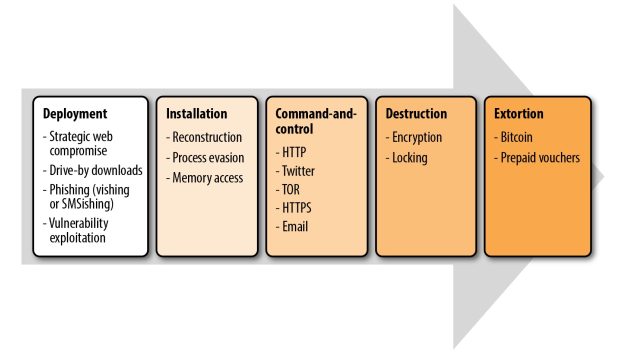
\includegraphics[width=\textwidth]{figuras/anatomy_of_a_ransomware_attack.png}
	\caption{Anatomy of a ransomware attack\cite{ransomware_oReilly}}
\end{figure}

\subsection{State of ransomware}
Ransomware is important for this project because it has gained much relevance in cybersecurity in the last years.
We think understanding it better is the first step to develop detection for it.
\linej
\linej
The main problems for studying ransomware is that is illegal and sometimes is hard to gather information.
For example most of the attacks are not reported and ransomware attacks are often analyzed offline and using auditing tools like decompilers because most of the time there is no source code\cite{ransomware_digital_extortion}.

\subsubsection{The growth of ransomware}
Next there are some estimations about the ransomware economy\cite{ransomware_economy}:
\begin{itemize}
	\item There are more than 6000 dark web marketplaces selling ransomware, with 45000 products listed.
	\item The ransomware marketplace on the dark web has grown in 2502\% from 2016 to 2017.
A major antimalware company states a 90\% increase in detection for business and a 93\% for individuals, in the same year\cite{ransomware_malwarebytes}.
	\item Some sellers of ransomware are making more than 100 thousand USD per year, just by retailing ransomware, when a legitimate software developer makes 30\% less.
\end{itemize}
\linej
Often ransomware includes remote control software to allow the remote execution of commands.
They often check if the server (certain ips or domains) can be reach before starting the process, waiting for a possible connection in the future if not.
Because these domain addresses are always resolving to new host ips, the criminal enterprises can regularly move around the Internet in relative safety, as they will always know their malcode can speak to them.
Keeping this Command and control server functional and anonymous may be hard and expensive depending on the approach used by the attacker.
They have evolved to use algorithms to generate a list of thousands of domains dynamically.
%Particularly DNS scans for new suspicious entries is advised.
\linej
The flaw of this approach is that can trigger behavioural alerts and reduces the scope of the attacks.
There is no need to initially contact the Command and control server, even for crypto ransomware because the public RSA key can be downloaded with the malware.
In some cases the attacker can command the malware to delete itself to avoid leaving evidence for security proffesionals\cite{ransomware_oReilly}\cite{ransomware_digital_extortion}.
\linej
\linej
The fundamental reason why this market exists is because the victims are willing to pay.
Is hard to know specifics because is estimated that most of the times these attacks are not reported (fewer are prosecuted and fewer are sentenced), but the mean crypto ransom is 300 USD per computer\cite{ransomware_digital_extortion}.
\linej
\linej
Unlike many other forms of cyberattacks, ransomware can be quickly and brainlessly deployed with a high probability of profit nowadays.
It has been a revelant type of malware since its beginning 23 years ago, but in the last years its economy has grown hugely, mainly because\cite{ransomware_digital_extortion}\cite{ransomware_economy}:
\begin{itemize}
	\item Bitcoin and Tor: for pseudo-anonymous activities.
	\item Proliferation of service providers: anyone can get into the ransomware business because technical knowledge is not needed for every step of the process.
	\item Lack of fundamental security controls: such as backups, penetration testing, patching, etc.
\end{itemize}
\linej
Bitcoin allows money to be transferred in a way that makes it nearly impossible for law enforcement to follow the money trail.
Anyone can set up a free and unrestricted Bitcoin wallet address without needing any approval from financial institution, regulations, or dealing with providing evidence and proofs of identity, taxation, evidence of residence, and so on.
Anybody can see the Bitcoin transactions or the flow of the cryptocurrency from address to address in the blockchain, making it possible to backtrack it to a real identity.
Unfortunately cybercriminals use to mix transactions to make them very hard to follow, this is what Bitcoin mixing services are for.
\linej
Tor is an anonymity network, that can be used to mask illicit activities and can be used just by running a program.
\linej
Neither provides perfect anonymity, but both are very easy to use, which has lowered the risk and barrier to entry for ransomware perpetrators.
The requirement for ransoms to be paid over the Tor network has ensured there is no centralized endpoint to investigate with traditional geo-based law enforcement approaches\cite{ransomware_digital_extortion}.
\linej
\linej
Due to these innovations, the underground ransomware economy is now an industry that resembles commercial software. It can be divided into sections like: development, support, distribution and even help desks. This market can be divided into tiers\cite{ransomware_economy}:
\begin{itemize}
	\item Authors: They can be responsible for the creation of the malware (including frameworks) and training and support on them. In the current state of the market they can just remain as authors, without ever running the malware in other computers. The cost is based on how customized the code is for a particular target.
	\item RaaS: Ransomware-as-a-Service borrows from the Software-as-a-Service model. RaaS is designed to make ransomware available to even novice criminals. It provides technical and step-by-step information on how to launch the ransomware attack with the purchased software. The most sofisticated have a platform for checking the current status of the attack. In some cases the ransom is split among the members of the supply chain.
	\item Distributors: A high profit/risk tier. They can distribute it themselves by spam campaigns, social engineering, targeted hacks or exploit kits. They can also leverage RaaS.
\end{itemize}
\linej
Splitting the work into different modules makes the ransomware market more complex and competitive.
It encourages role specialization (increasing quality and reducing risk for authors), it makes it easier to enter (expanding the market) and the modularity increases the quantity of different products (making the malware change faster).
\linej
Of course making it easier to enter the market is a double edge sword, because it makes it easier for police to investigate.
Defenders have the inherent advantage of interrupting the entire attack if they can break or interrupt any link of the chain.
\linej
This market can be simplified into the next image:
\begin{figure}[H]
	\centering
	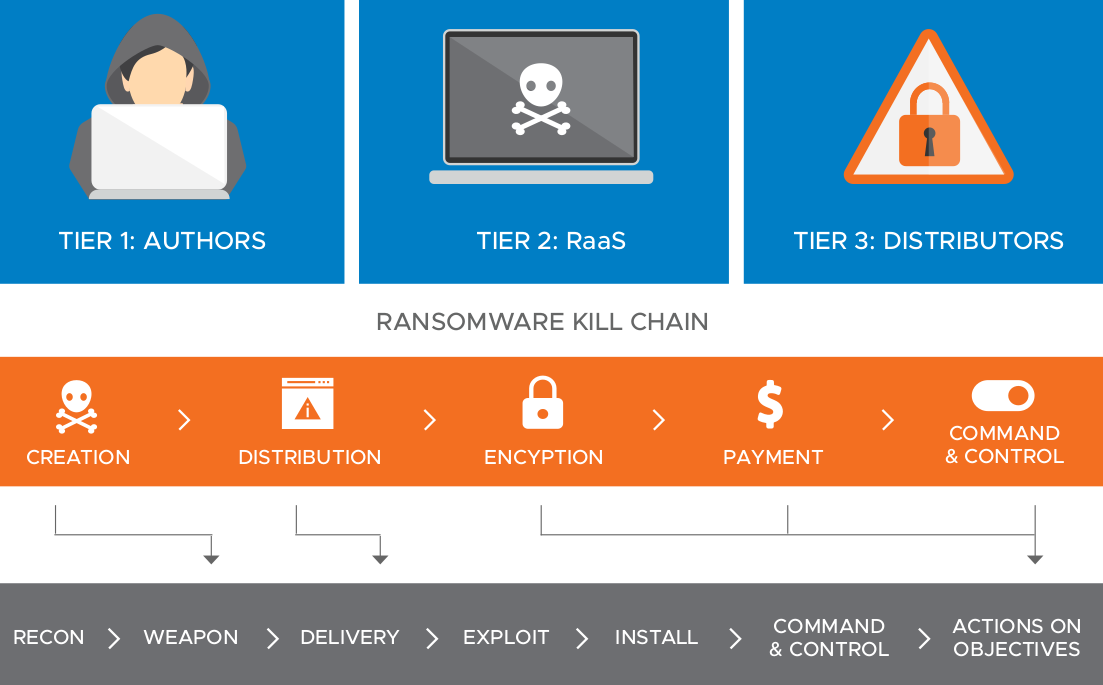
\includegraphics[width=\textwidth]{figuras/ransomware_chain.png}
	\caption{Ransomware supply chain and economy tiers\cite{ransomware_economy}}
\end{figure}
\linej
As long as the victims keep paying the ransom this trend will continue and the specialization will increase, resulting in more and bigger ransomware incidents.
%More creative forms of ransomware are sure to emerge over the years, like encrypting the master boot record\cite{ransomware_digital_extortion}.
The more ransomware is used the more secure the systems are against it, therefore in the future is also safe to assume that it would be more economical for criminals to use cryptominers or credential stealing instead\cite{ransomware_malwarebytes}.
\linej
\linej
Is also interesting to consider how ransomware and other attacks may take place if the main attack fails.
For example even if a ransomware attack fails it should be possible to use a distributed denial of service attack at greater cost and with lesser benefit.
A increase of malware as a distraction is expected in the future as the use and security of backups improves\cite{ransomware_economy}.

\subsubsection{Ransomware targets}
The more important the data the more money the victim is asked for.
Generally the bigger the business the better security it has and the more money cybercriminals can extort.
\linej
But the value of data may change from person to person, therefore there is no absolute best target for ransomware.
In the last years there has been an increase on the number of personal data sold in the dark web, which includes all kinds of data.
Cybercriminals can put pressure on the victim not only with direct ransom but also with the threat of selling the data.
\linej
In practice certain type of targets seems to rate higher on cybercriminals' priority lists\cite{ransomware_digital_extortion}:
\begin{enumerate}
	\item \textbf{Healthcare}: Apparently nothing sells as good on the black market as private healthcare records.
		Medical records do not lose value over time and they contain not only the person's medical history, but offers a full set of sensitive data that can be exploited in more ways than one (credit card numbers, social security numbers, banking credentials, e-mail IDs and employment history).
Cybercriminals use this currency to spread infections by phishing attacks, data fraud, and theft of medical histories.
	\item \textbf{Manufacturing}: Including businesses like automotive, electronics, textile and pharmacy.
The nature of the chemical and automotive businesses makes certain aspects horrifying, however, cybercriminals' motivation is predominantly financial, as they attack corporations not with the intention of mass murder, but to obtain valuable data and lucrative sensitive information.
	\item \textbf{Financial services}: The accessibility of payment methods and globally spread banking services whose main purpose is customer convenience will keep the financial industry high on the list. Attackers only need to impersonate or trick the victim in order to gain access to an account.
	\item \textbf{Goverment agencies}: They hold all types of personal and confidential data. If a goverment agency stops working it can affect many people.
	\item \textbf{Transportation}: Usually ransomware attacks set a time limit to pay the ransom, but in transportation real life sets the time limit. A higher effortless pressure results in less advance malware needs, meaning that transportation businesses could be effectively extorted with locker ransomware or denial of service attacks.
As in previous cases there is also interest in personal data and financial accounts.
	\item \textbf{Home users}: Ransomware is one of the best effective malware against personal computing users, who are considerably not experienced in cybersecurity.
This has increased due to the rise of smartphones and IoT devices.
Most users either don't use backups, they are not done often enough or they are stored in the same computer.
\end{enumerate}
\linej
In the end the target is always the people and the cybercriminal can either create a situation where is cheaper to pay or to gamble on the feelings (fear, shame, guilt, etc) of the victim.
\begin{figure}[H]
	\centering
	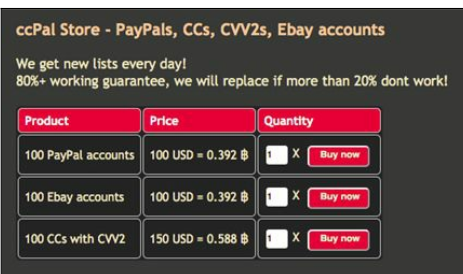
\includegraphics[width=.7\textwidth]{figuras/credit_cards_for_sale.png}
	\caption{Credit cards for sale\cite{ransomware_digital_extortion}}
\end{figure}

\section{Common patterns in crypto ransomware}
64\% of ransomware detected in 2016 was crypto ransomware\cite{ransomware_digital_extortion}, but it was not until 2013 that cybercriminals came back to it as their primary source of ransomware income\cite{ransomware_oReilly}.
The are many different crypto ransomware products, but we take interest in those who encrypt the files because, they are the ones that make the most impact on them.
If the encryption is done with strong algorithms it should not be possible to decrypt them in a lifetime (without knowing the decryption key).
\linej
\linej
This means suspicious activity regarding backups and files is common among the different crypto ransomware variants.
We assume the attacker prefers to execute the attack as fast as possible because:
\begin{itemize}
\item Once the encryption process starts is probably going to be detected very fast, either by an user or by an antimalware detector.
\item The only advantage of waiting is keeping the noise down.
\item If the encryption is only done on key files it should be very fast.
\item The system can be scanned quite silently before starting the encryption.
\end{itemize}
\linej
The most eficient way to encrypt the files is to use a symmetric algorithm (like AES-256), ensuring very strong and fast encryption even for big files.
The symmetric key is the same for encryption and decryption, and in this type of attack it holds the entire value of the ransom: once the ransom is paid the symmetric key is send to the victim to decrypt the files.
\linej
Obviously this key has to be kept secret by the attacker, therefore is ciphered with a public-key asymmetric algorithm (like RSA), allowing the attacker to transfer it without any risk.
Only the people with the private key should be able to decipher the symmetric key, therefore only the attacker can decipher it.
The public key is either downloaded with the malware or after the installation.
\linej
A major disadvantage of symmetric key encryption is that, in some cases, the key can be retrievered from RAM using special software.
Fortunately the DRAM in most systems is still live for anywhere from a few seconds to a few minutes after power loss, allowing a shutdown to stop the attack and still being able to recover from it.
However these techniques are unlikely to work with functions that avoid leaving trails in memory\cite{ransomware_oReilly}.
\linej
\linej
Most ransomware families use the built-in Windows Crypto API to handle the encryption.
While this is not a process that can necessarily be blocked, it is a process on which a security team can be alerted.
The problem is not detecting its use, but rather not spawning false positives\cite{ransomware_oReilly}.
\linej
\linej
Because the attack is supposed to be fast, the detection (and response) needs to be even faster to be able to stop it.
That is why multiple detection ways were explored for this case of study:
\begin{itemize}
\item For file encryption:
	\begin{itemize}
		\item Windows Defender's Controlled Folder Access
		\item Sysmon events
		\item Windows File Auditing
		\item Syscheck Monitoring with Wazuh
	\end{itemize}
\item For backup deletion:
	\begin{itemize}
		\item Detection of certain commands
		\item Increase of the backup volume free storage space
	\end{itemize}
\end{itemize}

\subsection{File encryption example}
This example shows how easily removal and encryption of files can be done with the right tools.
\linej
In this scenario the attacker uses AES for the files and ciphers the key passphrase with a RSA public key.
Both algorithms are supported by many tools: GnuGG, OpenSSL, custom DLLs and programming languages like PowerShell or Python.
OpenSSL was chosen because it works the same on Windows and GNU/Linux and is easy to use and install.
\linej
\linej
The first step would be the generation of the pair of RSA keys.
The private key stays in the computer of the attacker and the public key is stored into the victim's.
In this case the files are named ``keys.pem'' and ``public.pem'' respectively and the length of the key is 1024 bits.
The first file includes both private and public keys.
The second file is generated by the second command, which extracts the public key out of the combined file ``keys.pem''.
\begin{lstlisting}[style=PS,keywordstyle=\color{black}]
openssl genrsa -out keys.pem 1024
openssl rsa -in keys.pem -pubout -out public.pem
\end{lstlisting}
\linej
The next PowerShell script creates a random passphrase of letters, numbers and some special characters, which is used later for the symmetric key by the AES implementation of OpenSSL.
This passphrase is ciphered with the public RSA key and saved to the file ``passphrase.txt''.
Then script loops over all the files in \textit{C:/temp/} with the \textit{.txt} extension, encrypting them to AES-256 (in block cipher mode) and deleting the original file when done.
The \textit{openssl} variable is just for convenience.
\lstinputlisting[style=PS,caption=Script to encrypt files and cipher the passphrase with RSA,captionpos=b,label={lst:ransomware_basic}]{src/ransomware_basic.ps1}
\linej
The passphrase file can be deciphered with the private key, getting the random passphrase used in the script:
\begin{lstlisting}[style=PS,keywordstyle=\color{black}]
openssl rsautl -decrypt -in passphrase.txt -inkey keys.pem
\end{lstlisting}
\linej
Decrypting the files can be done using the same passphrase, because AES is a symmetric algorithm.
This example assumes the same value for the variables as in the encryption process:
\lstinputlisting[style=PS]{src/ransomware_decrypt.ps1}

\subsection{Detection of file crypto ransomware}
Next some sources for possible detection of crypto ransomware are examined.
Each of these options has its pros and cons, there is no restriction for using them toguether (in case one fails).
It is important to keep in mind that the Wazuh server is supposed to manage multiple systems, therefore scalability should be a concern and maybe only one of the solutions could be used in a real network.

\subsubsection{Windows Defender's Controlled Folder Access}
Windows Defender has the option to monitor specified folders for accesses and/or modification on real-time.
This feature is designed to combat the threat of ransomware.
It includes the option to whitelist applications and two basic modes of operation\cite{hardening_windows_10}:
\begin{itemize}
	\item Audit: Just notifies about suspicious activity with the event 1124.
	\item Block: Blocks and notifies about suspicious activity with the event 1123.
\end{itemize}
\linej
These events trigger for any suspicious activity, not only for ransomware attacks, but their detection is trivial \ref{lst:windows_defender}.
Windows Defender event log can be forwarded to Wazuh \ref{lst:forward_Windows_Defender}, allowing to improve the protection provided by Windows Defender with Wazuh.
The configuration of the whitelisted applications and the monitored directories can be managed by the Group Policy, the Windows Defender interface or the registry.
\linej
Windows defender has a set of monitored folders by default and the rest are listed in \textit{Computer{\textbackslash}HKEY\_LOCAL\_MACHINE{\textbackslash}SOFTWARE{\textbackslash}Policies{\textbackslash}Microsoft{\textbackslash}Win- dows Defender{\textbackslash}Windows Defender Exploit Guard{\textbackslash}Controlled Folder Access{\textbackslash}Pro- tectedFolders}.

\subsubsection{Sysmon events for file changes}
Sysmon events can be used to monitor changes in folders too, for example monitoring the folder \textit{C:{\textbackslash}temp{\textbackslash}}:
\begin{lstlisting}[style=xml]
<!--EVENT 2: FILE CREATION TIME RETROACTIVELY CHANGED IN THE FILESYSTEM-->
<FileCreateTime onmatch="include">
	<TargetFilename condition="contains">C:\temp\</TargetFilename>
</FileCreateTime>

<!--EVENT 9: RAW DISK ACCESS-->
<RawAccessRead onmatch="include">
	<Device condition="contains">C:\temp\</Device>
</RawAccessRead>

<!--EVENT 11: FILE CREATED-->
<FileCreate onmatch="include">
	<TargetFilename condition="contains">C:\temp\</TargetFilename>
</FileCreate>
\end{lstlisting}
\linej
Unfortunately none of the Sysmon events can detect file deletion, but they can be useful in other ways:
\begin{itemize}
	\item Event 2 could detect backdoors, which would change some key file and restore its previous creation time. Is not uncommon for ransomware to install them to extort the system in the future. Instead of relying on this event is a safer idea to use file integrity monitoring, checking the checksum of each key file for changes.
	\item Event 9 can be used to detect direct reading of the device, an alternative access method to avoid being detected by traditional file monitoring, like in the case of NinjaCopy \ref{invoke-NinjaCopy}.
	\item Event 11 can detect the new files, which could be identified as encrypted files in some cases with active response. Depending on the directory and the Wazuh rules there may be false positives.
\end{itemize}
%\linej
%For the execution of this example (with 4 .txt files) Windows Defender reported 6 events of type 1124 and Sysmon 5 of type 11 (4 creations of .txt.enc and symmetric.key).
%This makes sense because events 2 and 9 are triggered by change of creation time and raw access of the drive respectively.
%It is important to note that if the changes are blocked only events of type 1123 are generated.

\subsubsection{Windows File Auditing}
Windows File Auditing is a security feature that can be enabled and configured for multiple folders, reporting with events [4656-4663].
\linej
Windows does not log file activity in an usual way.
Instead, it logs granular file operations that require further processing and they are usually out of order.
The next table tries to describe and show the difference between these events as simple as possible\cite{windows_events}\cite{events_46_56_X}:
%\begin{table}[H]
	%\begin{tabularx}{\textwidth}{|l|X|X|}
		%\hline
		%\rowcolor{gray!30}
		%Event ID & Name and description & Useful data\\ \hline
		%4656& A handle to an object was requested. Logs the start of every file activity but does not guarantee that it succeeded.&
			%$\bullet$ Executable responsible
			%\linej $\bullet$ Filename of the object
			%\linej $\bullet$ Access mask
			%\linej $\bullet$ Accesses
			%\\ \hline
		%4658& The handle to an object was closed. Logs the end of a file activity.&
			%$\bullet$ Executable responsible
			%\\ \hline
		%4659& A handle to an object was requested with intent to delete. Logs a failed attempt to delete.&
			%$\bullet$ Executable responsible
			%\linej $\bullet$ Access mask
			%\\ \hline
		%4660& An object was deleted. Logs a delete operation.&
			%$\bullet$ Executable responsible
			%\\ \hline
		%4663& An attempt was made to access an object. Logs the specific micro operations performed as part of the activity.&
			%$\bullet$ Executable responsible
			%\linej $\bullet$ Filename of the object
			%\linej $\bullet$ Access mask
			%\linej $\bullet$ Accesses
			%\\ \hline
	%\end{tabularx}
	%\caption{Windows File Auditing events}
%\end{table}
\begin{table}[H]
	\begin{tabularx}{\textwidth}{|l|X|}
		\hline
		\rowcolor{gray!30}
		Event ID & Name and description\\ \hline
		4656& A handle to an object was requested. Logs the start of every file activity but does not guarantee that it succeeded.\\ \hline
		4658& The handle to an object was closed. Logs the end of a file activity.\\ \hline
		4659& A handle to an object was requested with intent to delete. Logs a failed attempt to delete.\\ \hline
		4660& An object was deleted. Logs a delete operation.\\ \hline
		4663& An attempt was made to access an object. Logs the specific micro operations performed as part of the activity.\\ \hline
	\end{tabularx}
	\caption{Windows File Auditing events}
\end{table}
\linej
More detail and thought is needed to complete the previous table\cite{windows_events}\cite{events_46_56_X}:
\begin{itemize}
	\item If an operation is rejected because not having enough privileges the only event issued is 4656.
	\item Windows only issues the event 4663 when the operation is complete. There might be multiple 4663 events for a single handle, logging smaller operations that make up the overall action.
	\item There are some events that do not appear in the previous range: 4657 is for registry changes and 4661 and 4662 are for AD objects.
	\item Events 4656 and 4663 include the ``accesses'' property, which refers to the type of operation: read, write, delete.
		The field can include multiple values, for example a rename involves read, delete and write.
		The problem of this field is that it does not follow a very normal interpretation of these types of basics operations.
	\begin{itemize}
		\item``WriteData'' implies that a file was created or modified unless a ``delete'' access was recorded for the same handle. The only way to know if it was created or if it was modified is to know if the file existed before, for example with a database.
		\item``ReadData'' is logged almost in every case, resulting in only being a normal read if none of the others are recorded.
		\item``Delete'' also includes move events. Move events do not spawn 4659 or 4660 events.
	\end{itemize}
	\item The path included in the event may be the device path, for example ``{\textbackslash}{\textbackslash}Device{\textbackslash}{\textbackslash}Harddisk- Volume3{\textbackslash}{\textbackslash}openssl{\textbackslash}{\textbackslash}bin{\textbackslash}{\textbackslash}bftest.exe'', instead of the normal volume path like ``c:{\textbackslash}temp''.
\end{itemize}
\linej
We can conclude that these events are not as easy to handle as they could be, but they can still be used for the detection of ransomware.

\subsubsection{Syscheck Monitoring with Wazuh}
Wazuh can check file changes directly checking checksum differences with the Syscheck module, this is known as File Integrity Monitoring.
Each agent maintains its own database for better performance.
\linej
The monitoring needs to be configured \ref{lst:syscheck_agent}\ in the agent, instead of the manager.
This generates Syscheck events that can be processed by rules, triggering alerts.
Syscheck has many options, like files to be ignored (which can also be done with rules) or the maximum recursion level to monitor.
\linej
The most interesting features of Syscheck for this project are\cite{libro_ossec}:
\begin{itemize}
	\item Real-time monitoring. It can only be set at folder level, not directly for files, but that can be worked around with ignores in fixed cases or match restrictions in rules.
	\item Scheduled scan. Interesting from a scalability point of view for checking security settings and looking for rootkits, but not useful for inmediate detection.
	\item Inmediate scan. The agent can be ordered to do a scan at any time. This is interesting to combine with active response.
	\item The creation and deletion of files can be detected too.
\end{itemize}

\subsubsection{Comparison of the different monitoring alternatives}
The previous analysis is interesting but a conclusion is yet to be reached.
Each of the next tables shows a simplification of the advantages and disadvantages of each of the examined methods:
\newcolumntype{w}{>{\hsize=.5\hsize}X}
\begin{table}[H]
	\begin{tabularx}{\textwidth}{|w|w|}
		\hline
		\rowcolor{gray!30}
		Advantages & Disadvantages\\ \hline
			$\bullet$ It allows the accesses to be blocked (in Block mode).
			\linej $\bullet$ It can detect any kind of creation, modification and deletion.
			\linej $\bullet$ False positives are uncommon.
			\linej $\bullet$ Provides abstraction to the end user. Windows decides which programs are legitimate.
			\linej $\bullet$ Legitimate whitelisting. Blacklisting can be implemented with rules in Wazuh.
			\linej $\bullet$ Fundamentally faster active response than Wazuh, which adds multiple steps to the direct response of Windows Defender in block mode.
		&
			$\bullet$ The logs do not include the filename, just the folder path.
			\linej $\bullet$ The logs do not explain the reason to find the event suspicious.
			\linej $\bullet$ The logs do not detail the kind of file event (creation, modification or deletion).
				%During the testing they always reported ``blocked from modifying''.
			\linej $\bullet$ It is an external program, therefore it can not be totally trusted to work on complex cases.
			\linej $\bullet$ It is one of the most and first denfensive programs targeted by attackers.
			\linej $\bullet$ The whitelisting may need manual adjustment, for example allowing the Wazuh agent.
			\\ \hline
	\end{tabularx}
	\caption{Advantages and disadvantages of file monitoring with Windows Defender}
\end{table}

\begin{table}[H]
	\begin{tabularx}{\textwidth}{|w|w|}
		\hline
		\rowcolor{gray!30}
		Advantages & Disadvantages\\ \hline
			$\bullet$ They can detect other malware approaches to the files.
		&
			$\bullet$ They can not be used to detect any kind of changes.
			\linej $\bullet$ Real malware can be hard to tell apart from false positives.
			\\ \hline
	\end{tabularx}
	\caption{Advantages and disadvantages of file monitoring with Sysmon events}
\end{table}

\begin{table}[H]
	\begin{tabularx}{\textwidth}{|w|w|}
		\hline
		\rowcolor{gray!30}
		Advantages & Disadvantages\\ \hline
			$\bullet$ They can be used to detect any kind of creation, modification and deletion.
		&
			$\bullet$ They can be too complex and counterintuitive. Following their flow requires composite rules in Wazuh.
			\linej $\bullet$ Lack of critical information in the logs.
			\linej $\bullet$ Real malware can be hard to tell apart from false positives.
			\\ \hline
	\end{tabularx}
	\caption{Advantages and disadvantages of file monitoring with Windows File Auditing events}
\end{table}

\begin{table}[H]
	\begin{tabularx}{\textwidth}{|w|w|}
		\hline
		\rowcolor{gray!30}
		Advantages & Disadvantages\\ \hline
			$\bullet$ They can be used to detect any kind of creation, modification and deletion.
			\linej $\bullet$ Diff is supported for text files.
			\linej $\bullet$ They always include critical information, like the filename and the program.
		&
			$\bullet$ Real malware can be hard to tell apart from false positives.
			\linej $\bullet$ The format of the events is not suited for field matching.
			\\ \hline
	\end{tabularx}
	\caption{Advantages and disadvantages of file monitoring with Syscheck events}
\end{table}
\linej
From these tables we can conclude that:
\begin{itemize}
	\item Fast local action is more suited to antivirus than IDS, therefore it makes sense to turn to Windows Defender for this feature. Further actions can still be implemented with Wazuh active response. For the others the active response is still possible, but slower.
	\item Windows Defender is the most attractive method to detect and stop the malware, but there are risks in only trusting Windows Defender.
	\item Because is hard to detect the creation of new files with the Windows File Auditing it makes sense to use the event 11 of Sysmon for this and likewise Sysmon can not detect file deletion which this security auditing can. But both have fundamental problems with false positives.
	\item Direct monitoring with Wazuh seems to be easier and more effective that combining Windows File Auditing with Sysmon.
	\item The Sysmon events 2 and 9 are always useful to find suspicious events with a low chance of false positives.
	\item Windows Defender detects the attack on its own, while the others need to relate multiple events in a short period of time with Wazuh's composite rules.
\end{itemize}

\subsubsection{Protecting Windows Defender}
If Windows Defender is chosen for protection against ransomware then it makes sense to improve the protection of Windows Defender because is very targeted by attackers.
This project can not afford much time on this task, but it can provide a solution for the most basic way to deactivate Windows Defender completely or just any of the features against ransomware.
The easiest way for an attacker to do this is to use the Windows registry, therefore enabling or disabling directly the functionality in question.
\linej
Access to the registry can be hardened, but in this case is assumed that not allowing to use access to registry editing tools is not enough to prevent an skilled attacker from doing so.
\linej
In the end this is a complex problem that does not only affect Windows Defender (the Wazuh agent is a similar case) and is impossible to fully solve, but measures can be taken nonetheless.
\linej
\linej
There may exist better ways to ``block'' registry changes, but none were found.
The objective is to assure that certain entries never are set to 1 and that other entries are always set to 1.
In the registry the value 1 often means the setting is enabled.
In this scenario we assume the system has the entries with the desired values from the beginning.
\linej
More specifically the entries to avoid being 1 are in \textit{HKLM{\textbackslash}SOFTWARE{\textbackslash}Policies {\textbackslash}Microsoft{\textbackslash}Windows Defender{\textbackslash}}:
\begin{lstlisting}[style=xml,frame=none]
	Spynet\SpyNetReporting
	DisableAntiSpyware
	DisableBehaviorMonitoring
	DisableOnAccessProtection
	DisableScanOnRealtimeEnable
\end{lstlisting}
\linej
And the entries to keep their value as 1 are in \textit{HKLM{\textbackslash}SOFTWARE{\textbackslash}Policies{\textbackslash}Mi- crosoft{\textbackslash}Windows Defender{\textbackslash}Windows Defender Exploit Guard{\textbackslash}Controlled Folder Access{\textbackslash}}:
\begin{lstlisting}[style=xml,frame=none]
	EnableControlledFolderAccess
	ExploitGuard_ControlledFolderAccess_AllowedApplications
	ExploitGuard_ControlledFolderAccess_ProtectedFolders
\end{lstlisting}
\linej
Wazuh can monitor the registry for changes, but not creation, and Windows also has auditing features that allow to monitor the registry, but Sysmon seems easier to configure.
Periodic checks for changes, in case an event report was lost, can easily be done in Wazuh with the remote command feature.
Other real-time checks could also be implemented, like ensuring the Windows Defender process is running as expected.
\linej
Monitoring the registry for creation/deletion, value changes and renaming can be done with Sysmon events [12-14] respectively.
In this case we only need to monitor a few entries \ref{lst:sysmon_events_registry}.
These events can be a bit odd:
\begin{itemize}
	\item The Windows registry can use a temporary name for an entry, at least when manually creating one with the graphical user interface.
	\item There is no need to change the value in order to spawn an event 13, the execution of a change command is enough.
	\item An entry can be created with the desired value directly, only spawning an event 13.
	\item In the case of renaming there may not be an event of id 14, but one of id 13 (with the old name) followed with an event of id 12 (with the new name).
\end{itemize}
\linej
This means that the easies way to manage them is to:
\begin{itemize}
	\item Delete or set to 0 the entries to avoid being 1. This should be triggered by any of the [12-14] events, except the event 13 when the value is set to 0 (to avoid recursion).
	\item Create and set to 1 the entries that always should be 1. It should only happen when the entry is deleted or renamed.
	\item Set to 1 the entries that always should be 1. It should only happen when the entry is changed.
\end{itemize}
\linej
The rules to accomplish this are very simple \ref{lst:rules_registry}.
The only detail that can lead to confussion is the use of the \textit{field} tag to filter the event id instead of using the \textit{if\_group} tag, which is because \textit{if\_sid} with \textit{if\_group} interact as a logical OR, but \textit{if\_sid} with \textit{field} interact as a logical AND.
\linej
These rules cover the previous cases toguether with the active response configuration \ref{lst:active_response_registry}.
\linej
\linej
The active response command is executed on the agent that triggered the alert, running a CMD script, which runs a PowerShell script.
Direct execution of PowerShell is not possible yet, but it is in the works.
This is documented from \ref{lst:change-registry-value_0}\ to \ref{lst:delete-registry}.
For undesired entries changing the value and the deletion can both be used.
%The first time the active response was enabled the deletion did not work because a lack of privileges, which should be solved with:
%\begin{lstlisting}[style=PS]
%icacls 'C:\Program Files (x86)\ossec-agent\active-response\bin\change-registry-value_0.cmd' /setowner SYSTEM
%\end{lstlisting}
%Oddly enough after a reboot it started to work, even without setting the owner to SYSTEM.
\linej
\linej
In this case the entries were grouped for both rules and active response scripts, therefore instead of executing the command for only the affected entry it is done for the whole group.
This could be solved in multiple ways:
\begin{itemize}
	\item Having an alert and active response command for each entry.
	\item Sending the affected entry name as an argument. This can not be done yet in Wazuh.
	\item Having the final PowerShell script check manually the status to only work on the affected entry.
\end{itemize}
\linej
None were implemented because there is no downside at this scale to just execute script for all the related entries.
The main problem with this approach is the management is harder than if it were centralized.
%https://github.com/wazuh/wazuh-ruleset/issues/155
	%3002 - Real time protection encountered an error and failed.
	%5001 - Real time protection is disabled
	%5004 - Real time configuration changed
	%5007 - The antimalware platform configuration changed
	%5010 - Scanning for malware and other potentially unwanted software is disabled.
	%5012 - Scanning for viruses is disabled.
	%5101 - The antimalware platform is expired

\subsubsection{Reducing false positives}
In this case the problem with detection methods other than Windows Defender's Controlled Folder Access is there is no guarantee that the reported events are from normal and legitimate operations.
There are many circumstancial solutions like: maintaining a list of allowed applications or looking for suspicious behaviour (for example many files created and later deleted in a short time).
But none of them are guaranteed to always work by default.
Instead a simpler approach was implemented: use decoys and look for suspicious behaviour.
Because Windows Defender does not provide the filename decoy filtering can not be used with it.
\linej
The deletion of files was chosen as the suspicious behaviour to detect, because there is no need to save the encrypted files in the same directory.
Mass creation of files can also be detected and identified as suspicious.
\linej
\linej
Decoy files are files that appear to be normal files but should never be changed or deleted by a legitimate user.
Therefore if there are such events paired with other suspicious behaviour in a short amount of time it should mean that a ransomware attack is going on.
\linej
These restrictions can be increased to reduce the chance of generating false positives at the risk of losing real positives.
Increasing the required number of other deleted files over the minimum of two \ref{lst:syscheck_rules_2}, for the decoys and Wazuh composite rules, in contrast with the normal rules \ref{lst:syscheck_rules}.
\linej
There are ways to hide decoy files for normal users and to automate their creation, but that is trivial and not the objective of this section.
To reduce the file storage used by the decoys hard links and soft links could be used, but there is no guarantee that ransomware would treat the files exactly as the rest, therefore reducing the chance of the detection to work.
\linej
In this example the decoys are just named ``decoy1'' and ``decoy2'' for simplification.
Two decoys are used instead of only one with a complex way to duplicate its alert (like using active response), because the storage space should not be affected by this and it is easier.
\linej
\linej
Decoys proved to work on testing with the encrypting script \ref{lst:ransomware_basic}\ and detection with both Windows File Auditing \ref{lst:file_audit}\ and Syscheck Monitoring with Wazuh \ref{lst:syscheck_rules}.

\subsection{Backup deletion}
Backups provide effective mitigation against crypto ransomware attacks in most cases.
There are many scenarios between distributed backups in servers accross the world and just having local backups.
Their ability to overcome ransomware attacks depends on multiple factors like: the exact malware, the distribution of the backup system, the security of the backup system, etc.
\linej
In this case we assume the target only has local backups that are managed with the Shadow Copy service, which allows files to be copied even when in use.
%A Shadow Copy storage can be added to a device and a Shadow Copy can be created as easily as:
%\begin{lstlisting}[style=xml]
%vssadmin add shadowstorage /For=C: /On=F: /MaxSize=50%
%vssadmin create shadow /For=C:
%\end{lstlisting}
%\linej
Some known ransomware like Locky and Cerber try to delete existing Shadow Copies before encrypting the files\cite{ransomware_oReilly}:
\begin{lstlisting}[style=PS]
C:\Windows\system32\vssadmin.exe delete shadows /all /quiet
C:\Windows\system32\wbem\wmic.exe shadowcopy delete
\end{lstlisting}
\linej
Only vssadmin was used for testing because wmic is just the same but from remote (and is even easier to detect because it has three specific Sysmon events).
A new disk was added to the virtual machine of the SMB server to serve as a Shadow Copy storage on the \textit{F:} drive.
This and a network disk are the most basic methods for scheduling backups using Shadow Copies, due to Windows restrictions.
\linej
\linej
It is not possible to detect the deletion of Shadow Copies with file monitoring methods like: Sysmon events, Windows' File Activity Monitoring events and Windows Defender's Controlled Folder Access.
The Shadow Copies are not in the filesystem of the volume, they are managed directly by the Shadow Copy service as special storage.
%TODO detection
%detectar borrado de backups mirando el tamaño libre en el volumen
	%si disminuye se actualiza (CBC database?)
	%si aumenta se debe de haber borrado algo


\subsection{Active response against ransomware}
%TODO


%TODO real ransomware tests
%\section{}
%TODO table detection Yes/No colors
%\begin{table}[H]
	%\centering
	%\begin{tabular}{|l|l|l|}
		%\hline
		%\rowcolor{gray!30}
		%Ransomware variant & Detected \\ \hline
		%TODO& \RYES\\ \hline
	%\end{tabular}
	%\caption{Real ransomware detection by previous methods}
%\end{table}

\section{Mitigation}
Ransomware does not need any particular weakness or vulnerability to work on a system, but the better protected the system is the harder it is for it to be victim of a ransomware attack.
Next are some of the most basics measures to mitigate ransomware attacks\cite{ransomware_oReilly}\cite{ransomware_digital_extortion}\cite{hardening_windows_10}:
\begin{itemize}
	\item Prevent the ransomware from accessing the Windows Registry:
Ransomware can use the registry to maintain persistence through reboots and to disable security features on the victim machine.
Administrators can disable writing to at least to certain registry keys using Windows Resource Protection.
	\item Cyber insurance:
In some cases it may reduce certain costs, like: notifications costs to data breach victims, loses from offline periods, legal defense costs and forensics and investigation costs.
	\item Using decoy resources:
They can be used to detect unplanned acceses or changes and to find vulnerable systems (using honeypots).
	\item Security awareness and education:
It is important to teach the basics of cybersecurity threats to its targets.
For example being careful with web browsing and everyday documents like PDFs or Mircrosoft Office documents, all of which can contain malware that runs on access.
	\item Fundamental security controls:
They provide the base for the cybersecurity of the system.
Their vulnerabilities may allow or increase the scope of all kinds of attacks.
They may change from system to system, but the basic are: backups, penetration testing, patching, software updates, firewall, antimalware software and advanced security options (like Exploit Protection, Secure Boot and Early Launch Antimalware).
	\item Granular permissions and isolation:
Minimizing the available administrator accounts to attackers, by reducing its number and keeping them as isolated as possible, is a good way to mitigate their threat.
For example it makes sense to require administrator privileges for the backup service, which is key for crypto ransomware, even when they are remote backups.
They can mean the difference between compromising just a system or the whole network, when a system becomes a central point of failure.
	\item Restrictions to unnecessary services and software:
They may not be enough to keep the attacker away from using the software, but at least they probably would rise some alerts or slow the process.
In some cases the attacker may reconsider the target to not be worth the effort.
Some of the recommended restrictions are over: Tor, powershell, vssadmin, wmic, certain directories and not digitally signed software.
	\item Removing unused devices:
Basic action to prevent possible further infection spreading.
It should be applied to physical devices like: mapped drives, USB storage devices or memory sticks and smartphones.
All writeable devices should be removed from a station when not in use.
	\item File exchange management:
Many businesses need file sharing to worked on collaboratively.
Once the process of file sharing becomes a routine, security gets on wobbly feet.
To keep the filesystem safe, organizations should establish best practices for sharing data and files in a safe and secure manner.
An effective way to minimize risks is application of digital signatures.
	\item Response plan development:
At a moment of crisis, decision-making can be weak exacerbating the consequences of the infection.
Developing a solid plan for fighting malware infections is the first mitigation task that should be completed by the responsible business leaders in the organization.
\linej
Next is a quick five-step guide for businesses under attack:
	\begin{itemize}
		\item Disabling sync features:
Enabled syncing features makes it easier for offenders to instigate attacks that will overwrite files, especially when they use crypto ransomware.
By disabling sync features you can prevent targeting data in the cloud.
		\item Removing malware from the affected devices:
There are two basic ways to do this: scan the systems or replicate the system from scratch.
The first option is usually faster but there is no 100\% guarantee to detect the malware, while the second needs preparation beforehand (for example with backups) and time with services unavailable.
Replicate the system from scratch can be much more easier and faster with virtualization management.
		\item File recovery:
Depends on the system version in use and there may me data that can not be restored.
		\item Blocking the payment transaction:
Under certain circumstances, the payment transaction can be blocked, even if you have already started the payment process.
This is throughble when the files have been successfully recovered without using the help provided by the attackers.
		\item Contacting law enforcement and reporting the crime:
It is important not only for taking action in the concrete case, but also for predicting and protecting against future cases.
Sending a report to the relevant software authorities is also recommended.
If there were more reports then there would be more data on ransomware attackes, making it easier to defend against it.
	\end{itemize}
\end{itemize}


%\section{Conclusion}
%TODO

